\chapter{Diagram class}

\section{User Interface}
		\subsection{Web}
		
\section{HTTP}
%begin core diagram
\newpage
\section{Core}
	\subsection{Exercise}
		\begin{figure}[ht]
			\begin{center}
				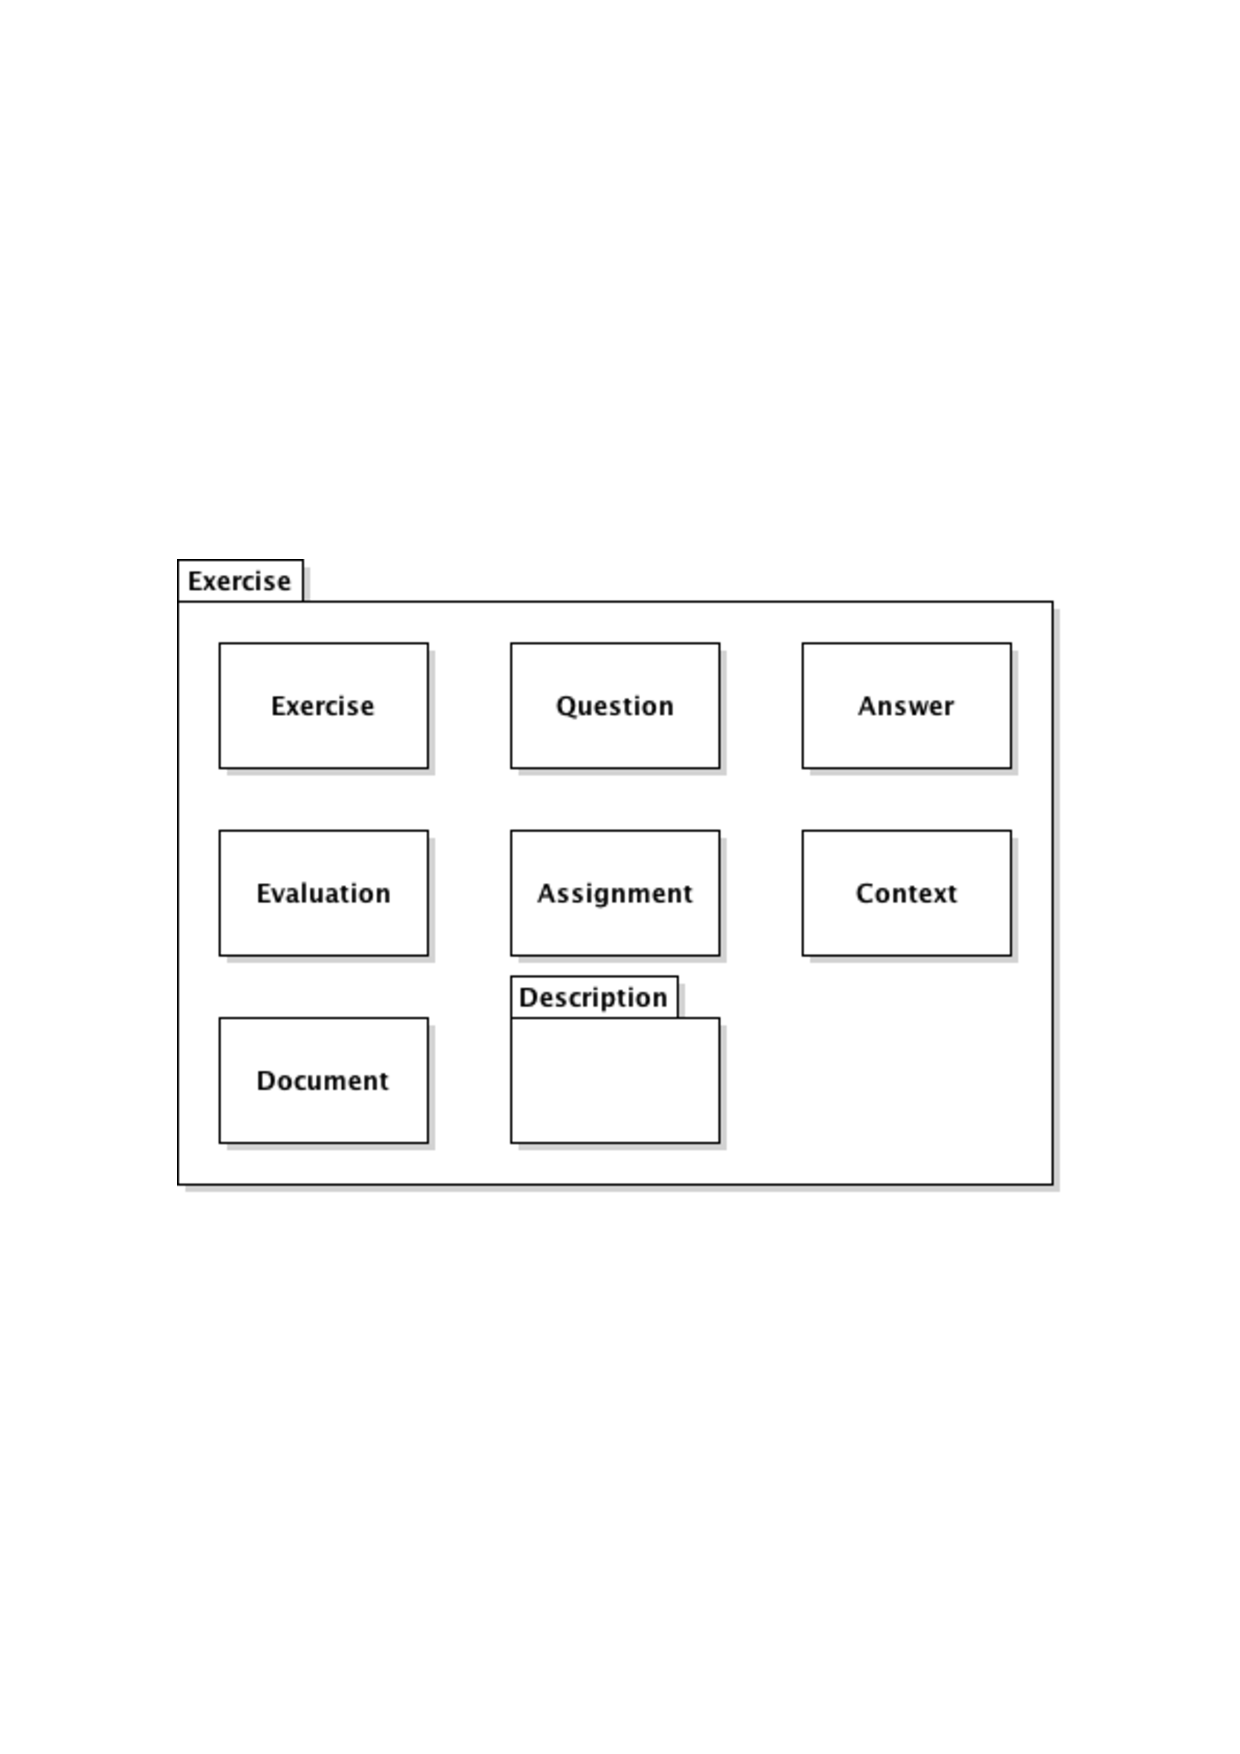
\includegraphics[width=\textwidth,  trim=2cm 9cm 2cm 9cm]{UML_figure/DC/core/exercise/DC_Exercise.pdf}
				\caption{Core diagram class : Exericse}
			\end{center}
		\end{figure}
		\subsubsection{Exercise} 
			This module implements an exercise entity.
		\subsubsection{Question}
			????
		\subsubsection{Answer}
			This module implements an answer entity part of a question
		\subsubsection{Evaluation}
			This module implements an evaluation entity on exercises.
		\subsubsection{Assignment}
			This module implements a priority entity on exercise for students.
		\subsubsection{Context}
			This module implements a context for an evaluation.
		\subsubsection{Document}
			????
	\subsection{Exercise : Description}
		\begin{figure}[ht]
			\begin{center}
				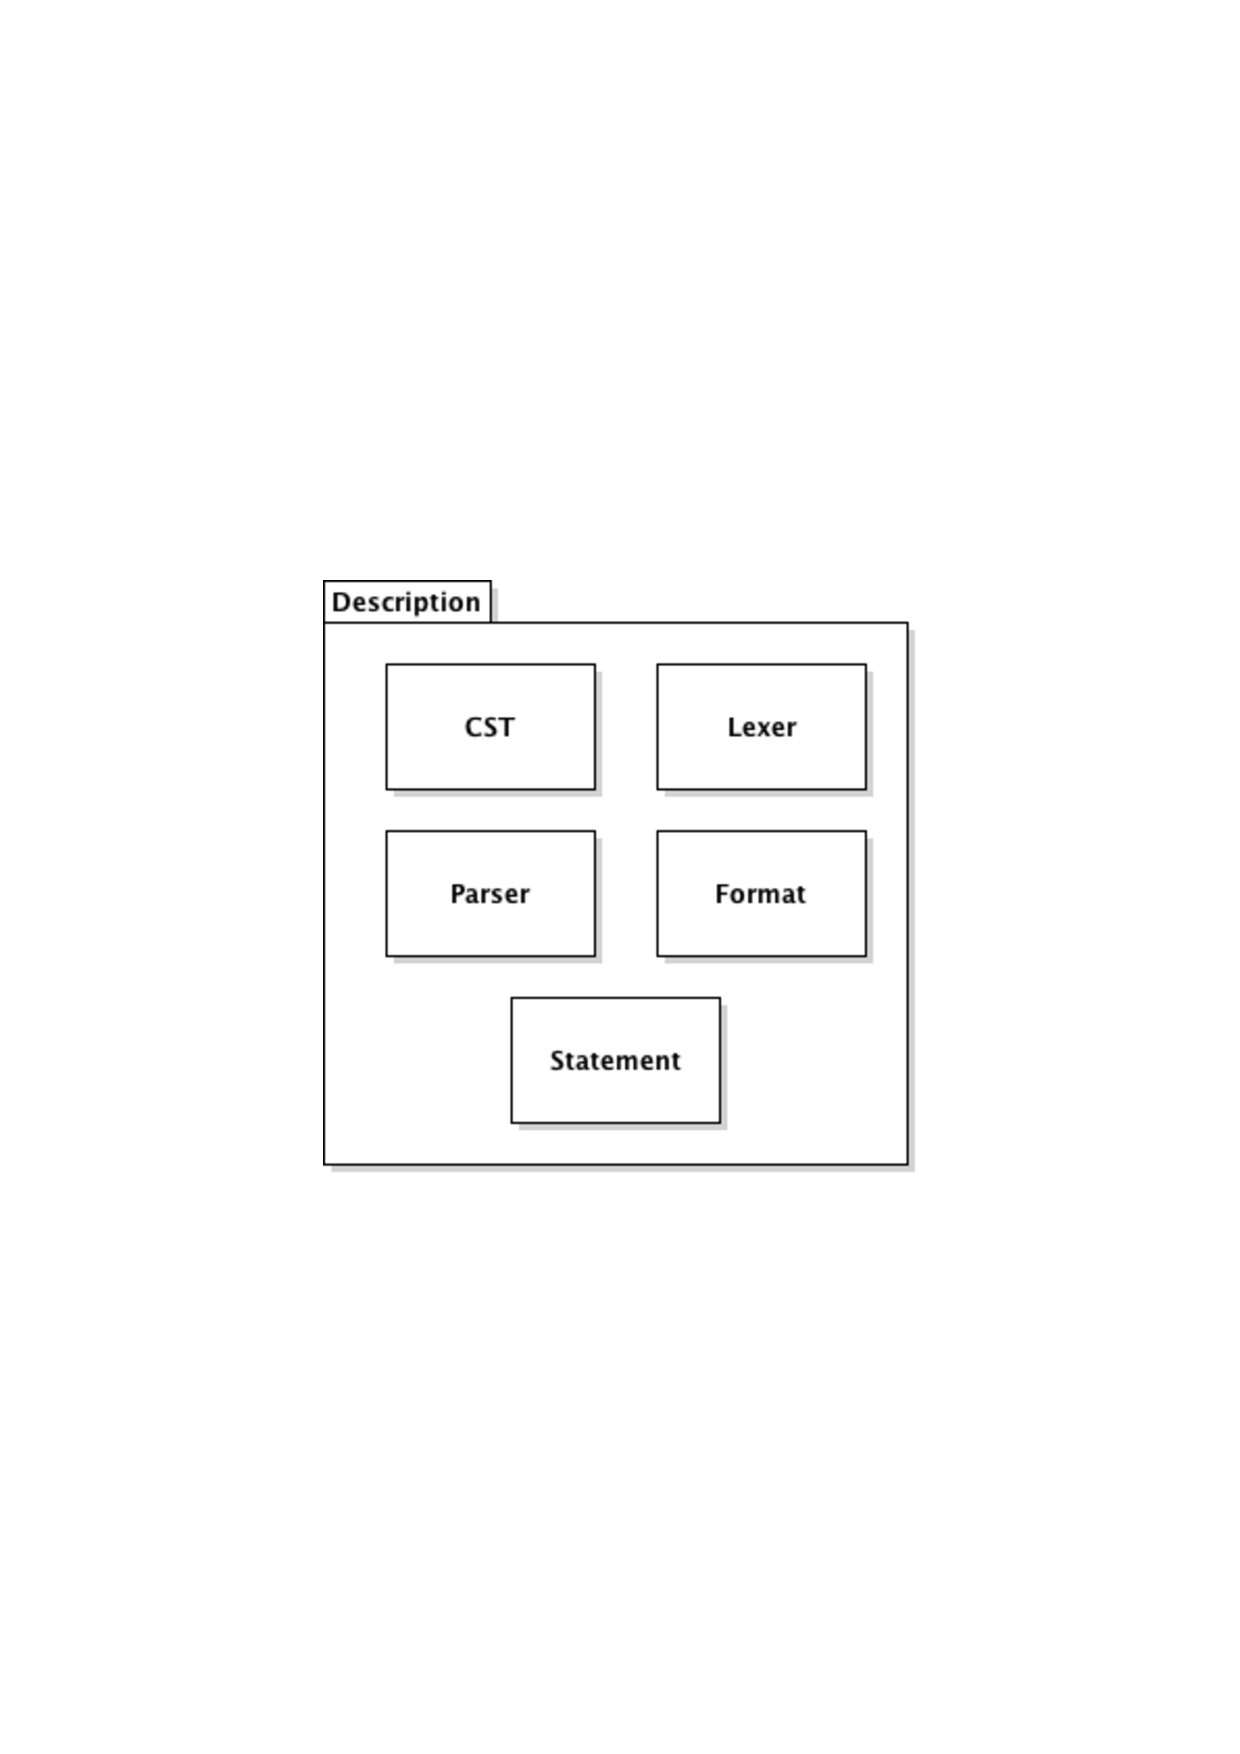
\includegraphics[width=\textwidth,  trim=2cm 10cm 2cm 9cm]{UML_figure/DC/core/exercise/DC_Description.pdf}
				\caption{Core diagram class : Exercise - Description}
			\end{center}
		\end{figure}
		\subsubsection{CST}
			This module implements the syntax rules for a statement.
		\subsubsection{Lexer}
			This module implements rules for the lexer.
		\subsubsection{Parser}
			This module implements rules for the parser.
		\subsubsection{Format}
			This module implements a parser for a description.
		\subsubsection{Statement}
			???? 
\newpage
	\subsection{Machinist}
		\begin{figure}[ht]
			\begin{center}
				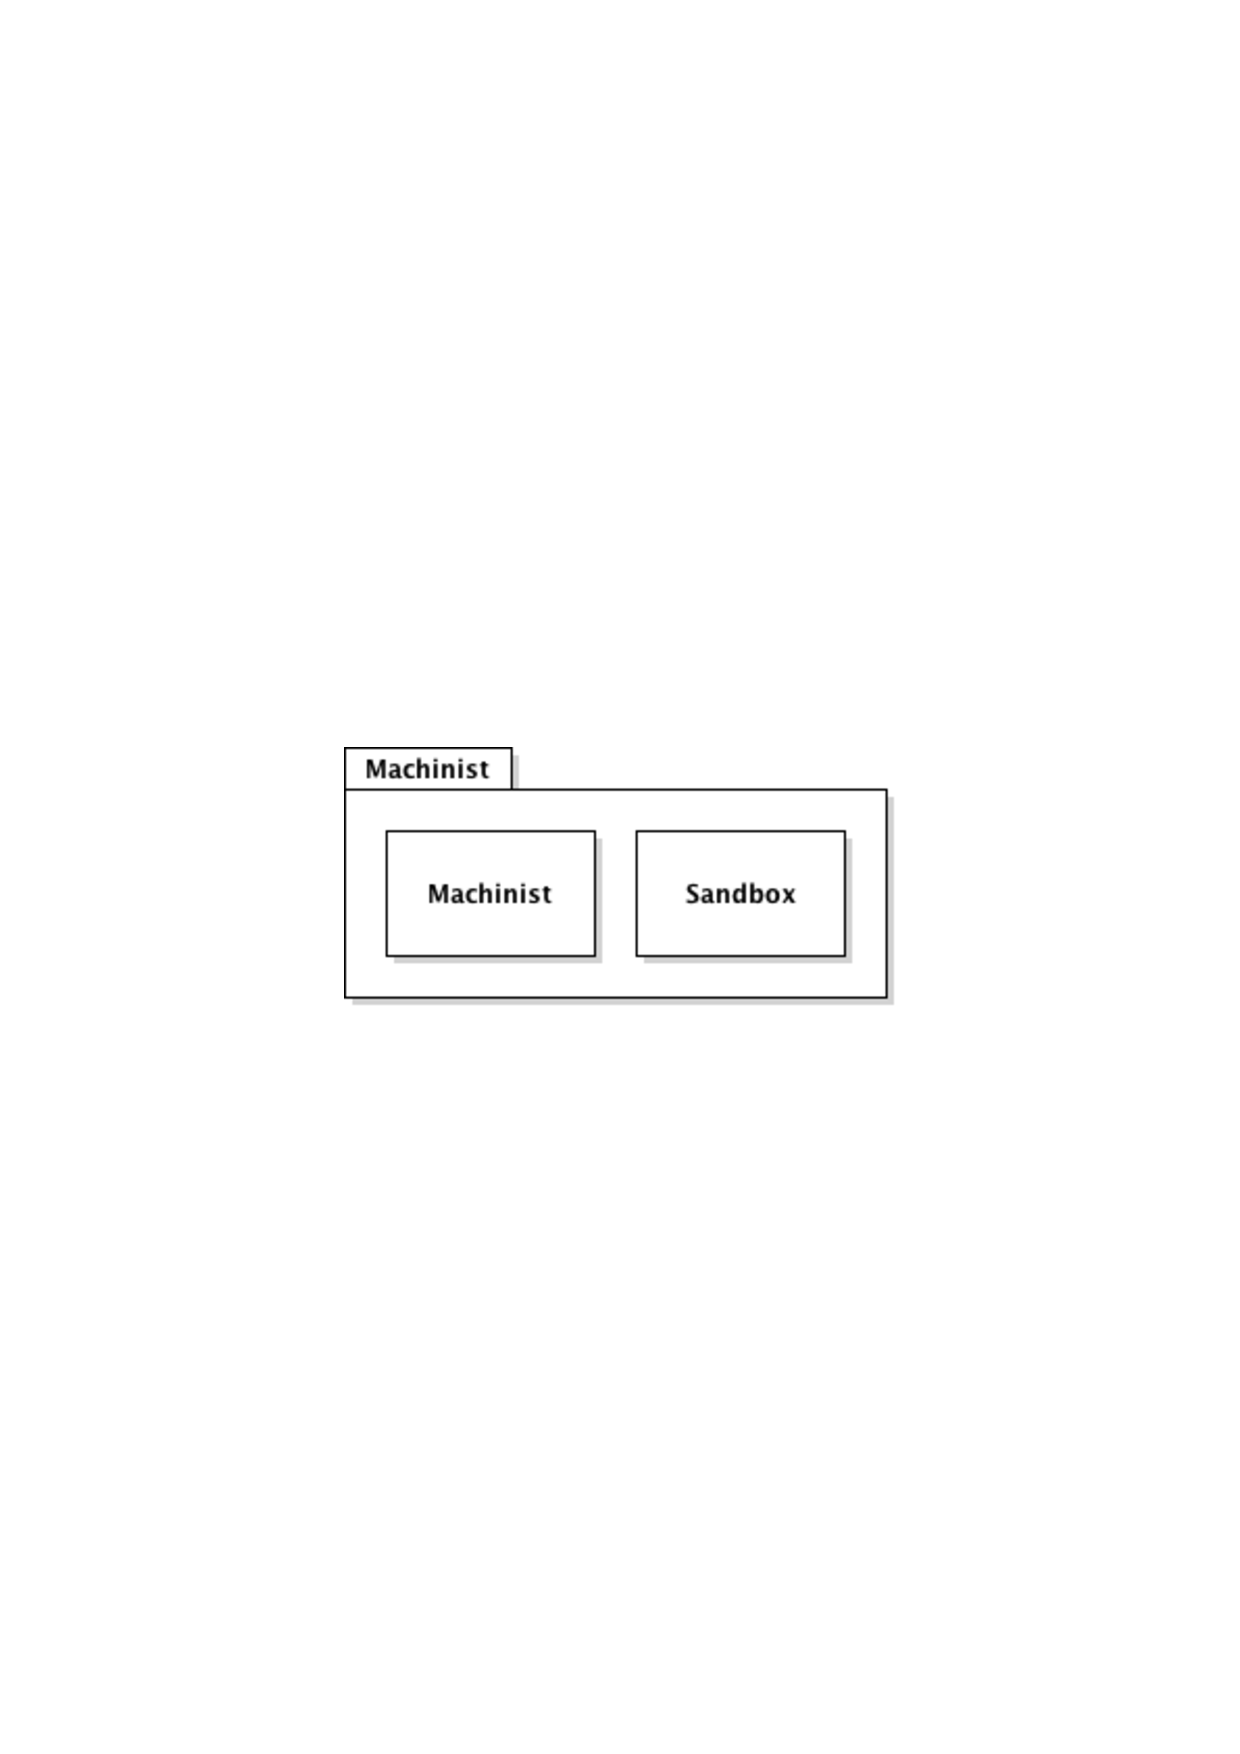
\includegraphics[width=\textwidth,  trim=2cm 12cm 2cm 12cm]{UML_figure/DC/core/machinist/DC_Machinist.pdf}
				\caption{Core diagram class : Machinist}
			\end{center}
		\end{figure}
		\subsubsection{Machinist}
			This module implements a sandbox provider.
		\subsubsection{Sandbox}
			This module implements an abstraction on environment used for the sandbox. 
	\subsection{Reactive}
		\begin{figure}[ht]
			\begin{center}
				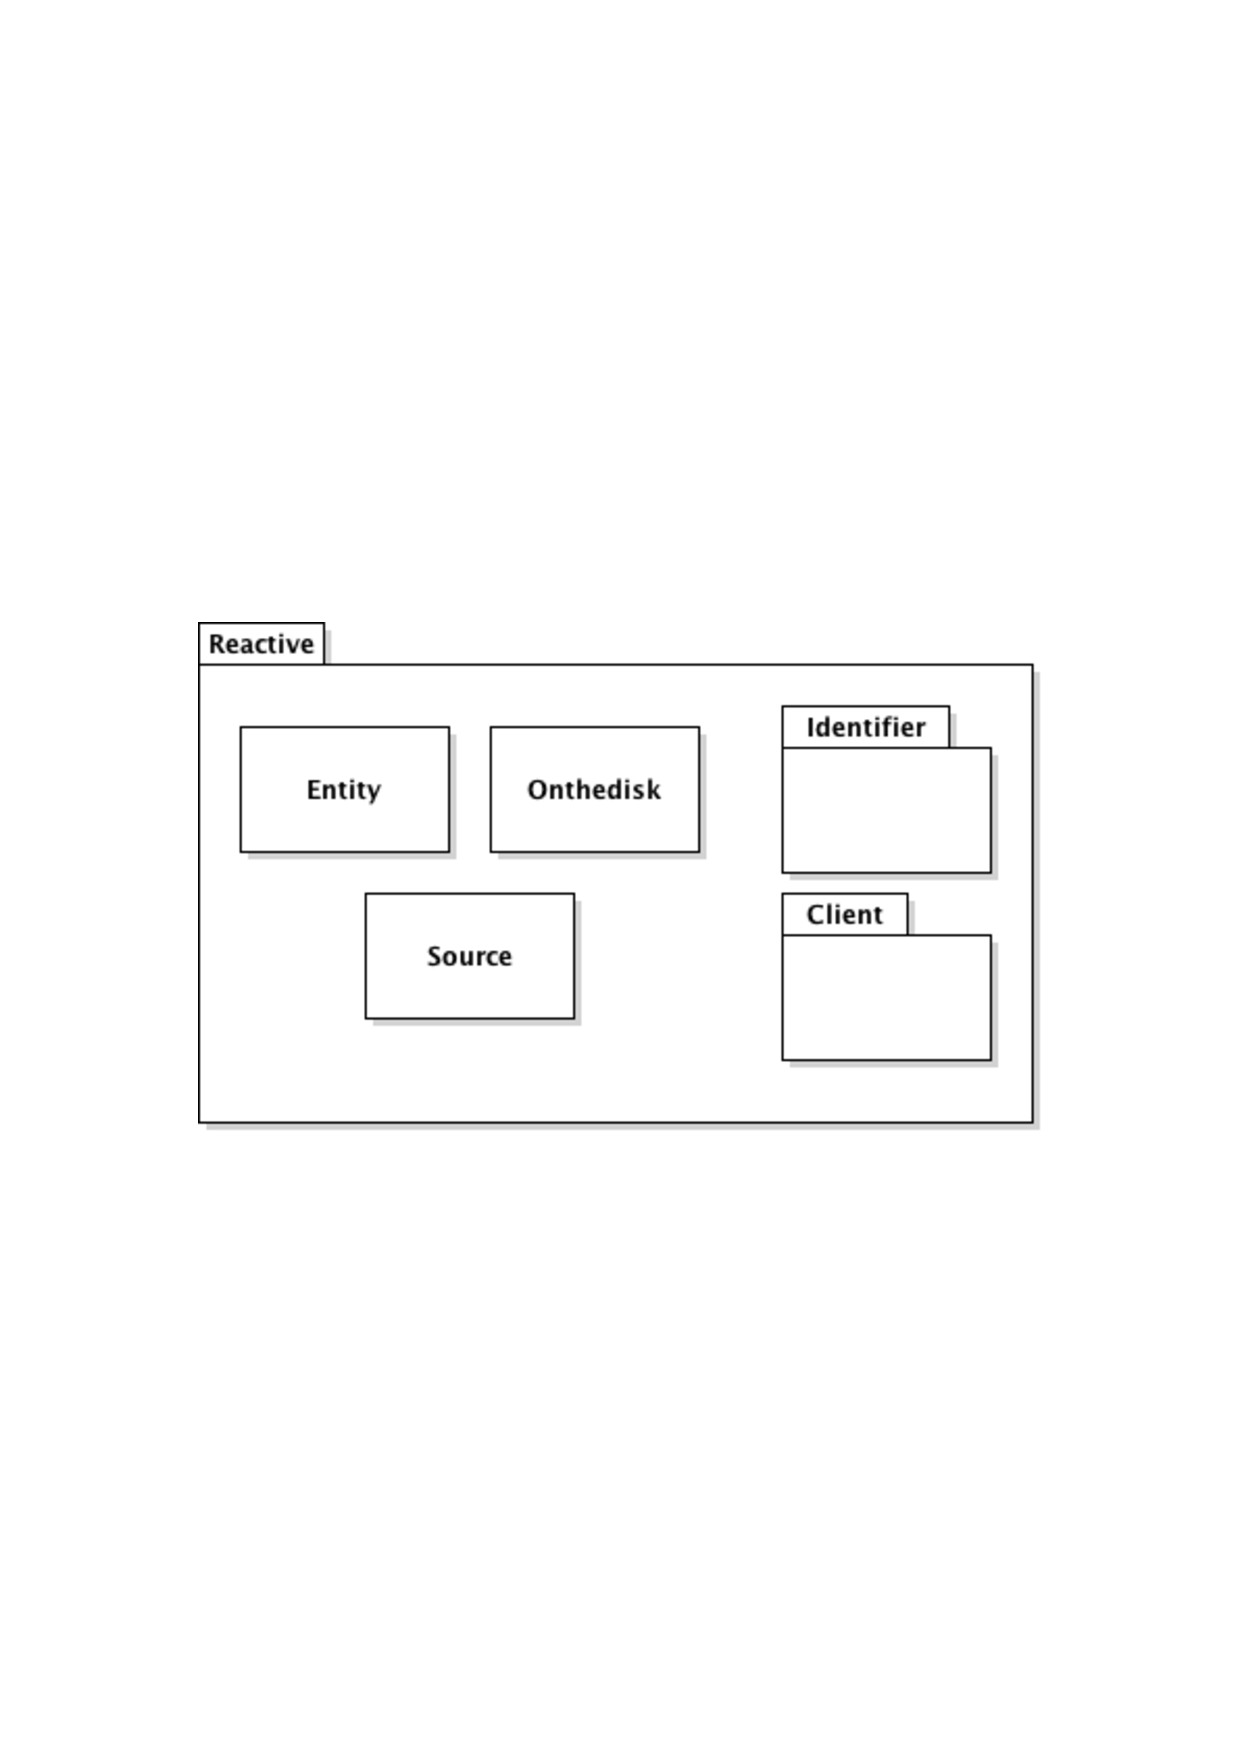
\includegraphics[width=\textwidth,  trim=2cm 10cm 2cm 10cm]{UML_figure/DC/core/reactive/DC_Reactive.pdf}
				\caption{Core diagram class : Reactive}
			\end{center}
		\end{figure}
		\subsubsection{Entity}
			This module implements a reactive entity.
		\subsubsection{Onthedisk}
			This module implements an entity state to be serialized.
		\subsubsection{Source}
			This module implements a system which associates a filename with a content.
	\subsection{Reactive : Identifier}
		\begin{figure}[ht]
			\begin{center}
				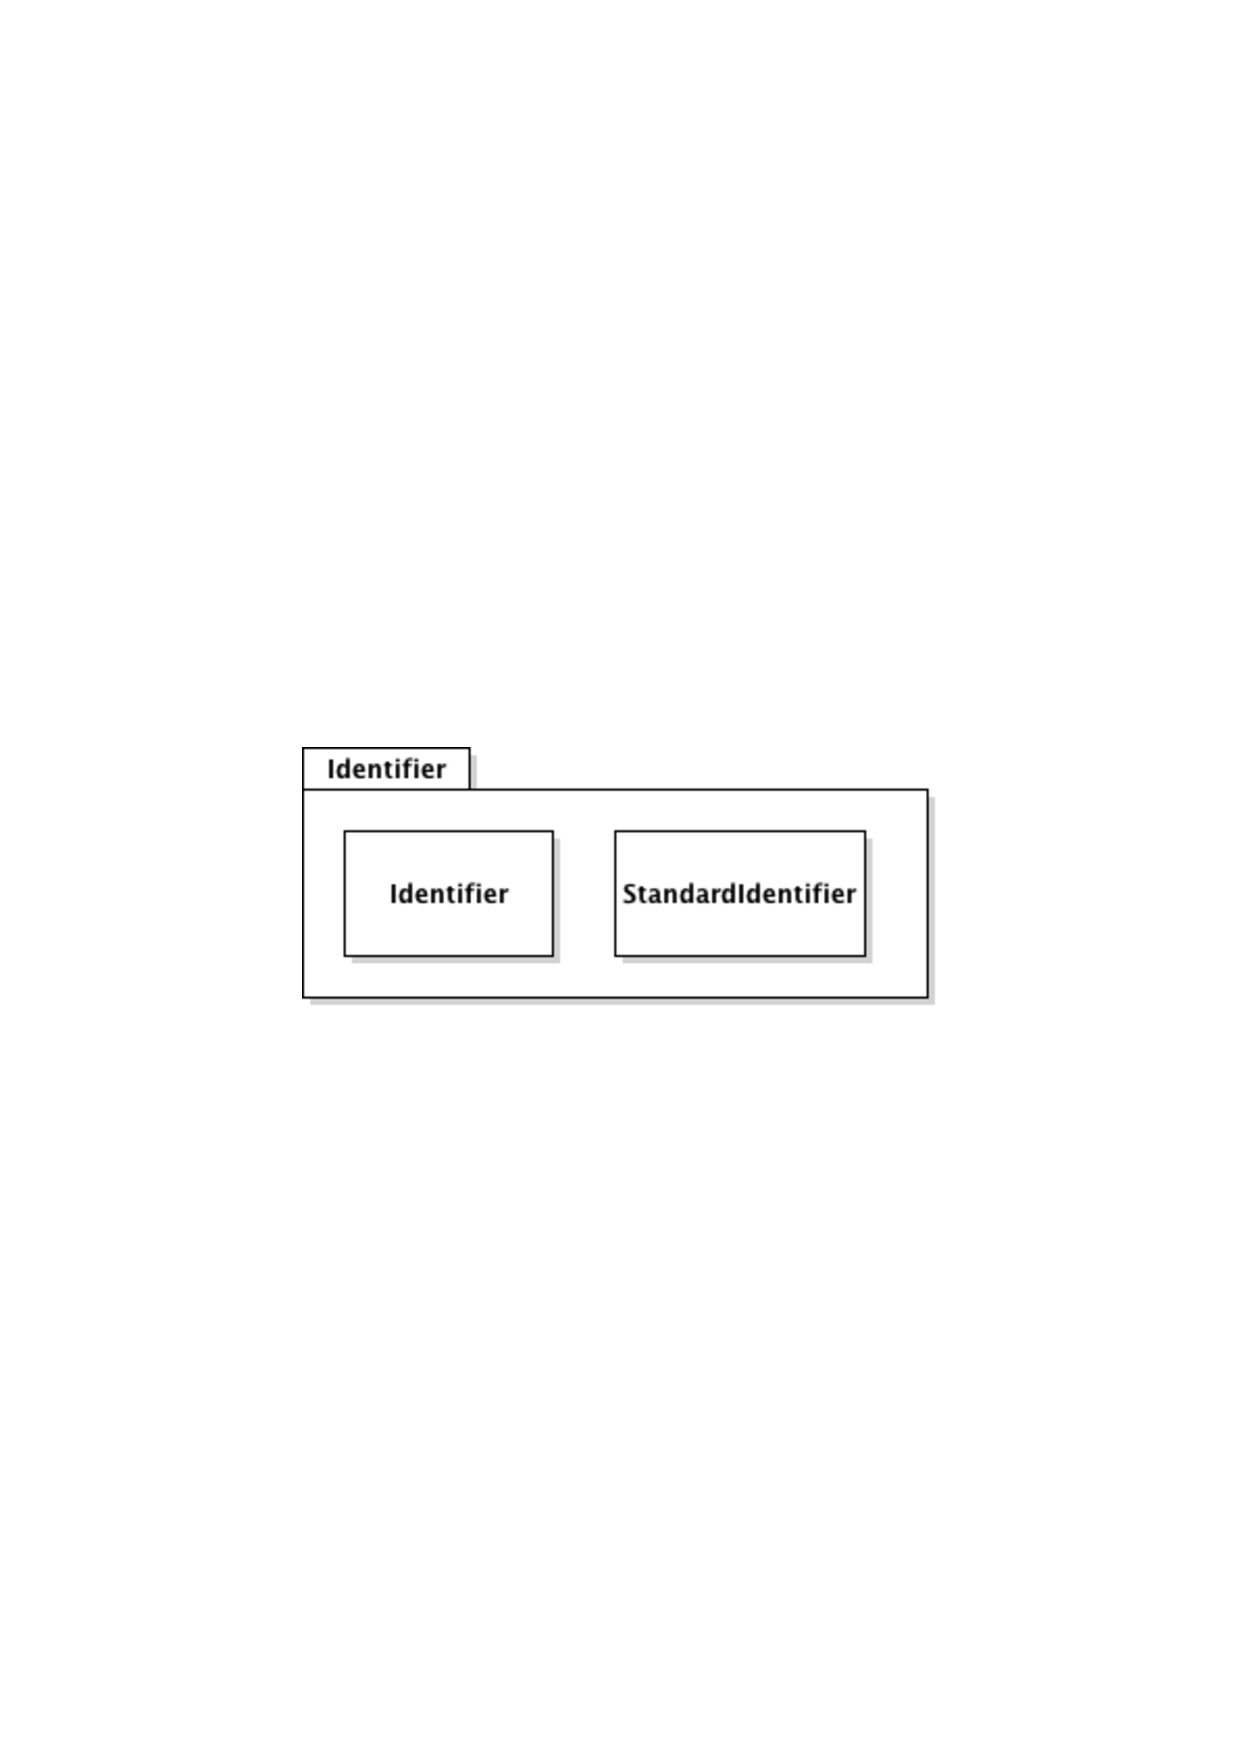
\includegraphics[width=\textwidth,  trim=2cm 12cm 2cm 12cm]{UML_figure/DC/core/reactive/DC_Identifier.pdf}
				\caption{Core diagram class : Reactive - Identifier}
			\end{center}
		\end{figure}
		\subsubsection{Identifier}
			This module implements an identifier for a reactive entity.
		\subsubsection{StandardIdentifier}
			This module implements a standard identifier for reactive entities. 
\newpage
	\subsection{Reactive : Client}
		\begin{figure}[ht]
			\begin{center}
				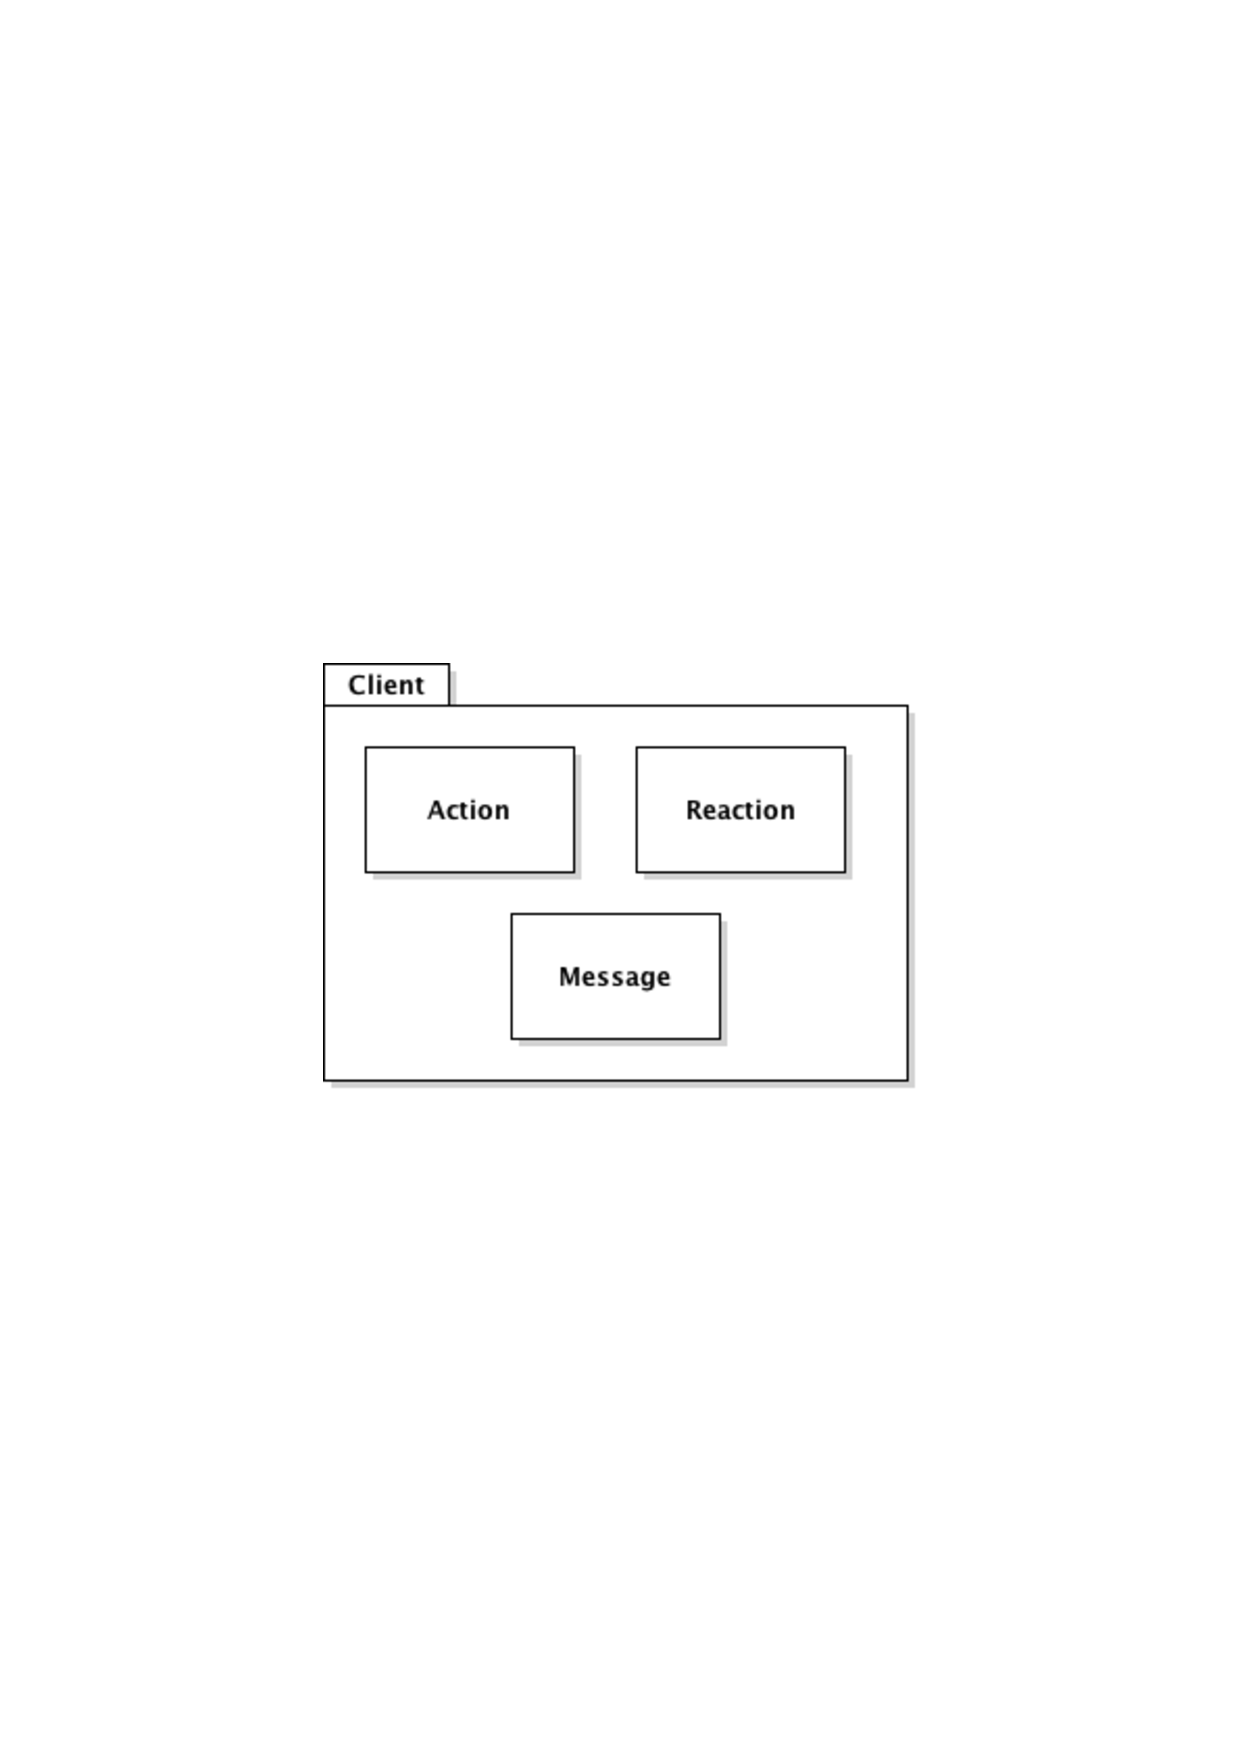
\includegraphics[width=\textwidth,  trim=2cm 11cm 2cm 10cm]{UML_figure/DC/core/reactive/DC_Client.pdf}
				\caption{Core diagram class : Reactive - Client}
			\end{center}
		\end{figure}
		\subsubsection{Action}
			This module implements an association with a process and a client.
		\subsubsection{Reaction}
			This module implements a communication channel between the server and the client.

	\subsection{User}
		\begin{figure}[ht]
			\begin{center}
				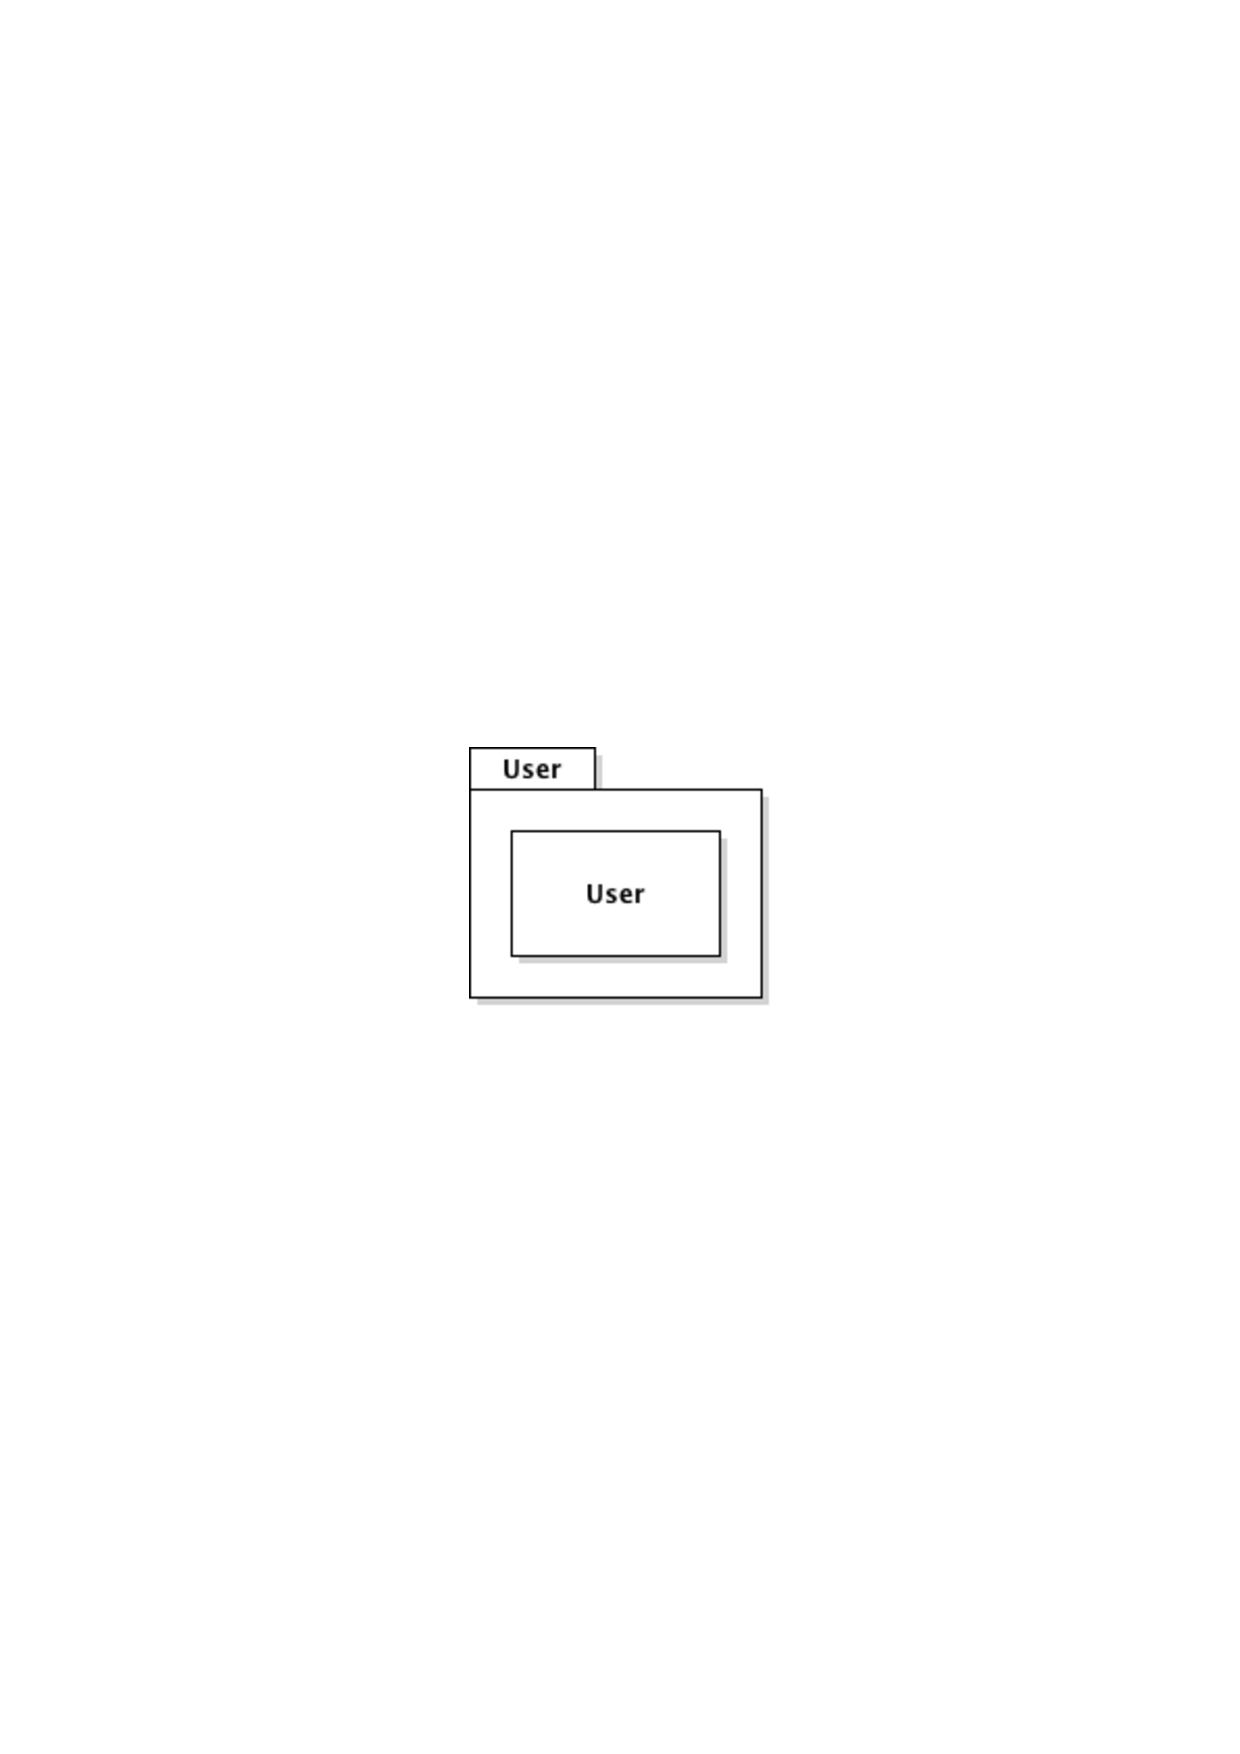
\includegraphics[width=\textwidth,  trim=2cm 12cm 2cm 12cm]{UML_figure/DC/core/user/DC_User.pdf}
				\caption{Core diagram class : User}
			\end{center}
		\end{figure}
		\subsubsection{User}
			This module implements an user entity.
\newpage
	\subsection{Config}
		\begin{figure}[ht]
			\begin{center}
				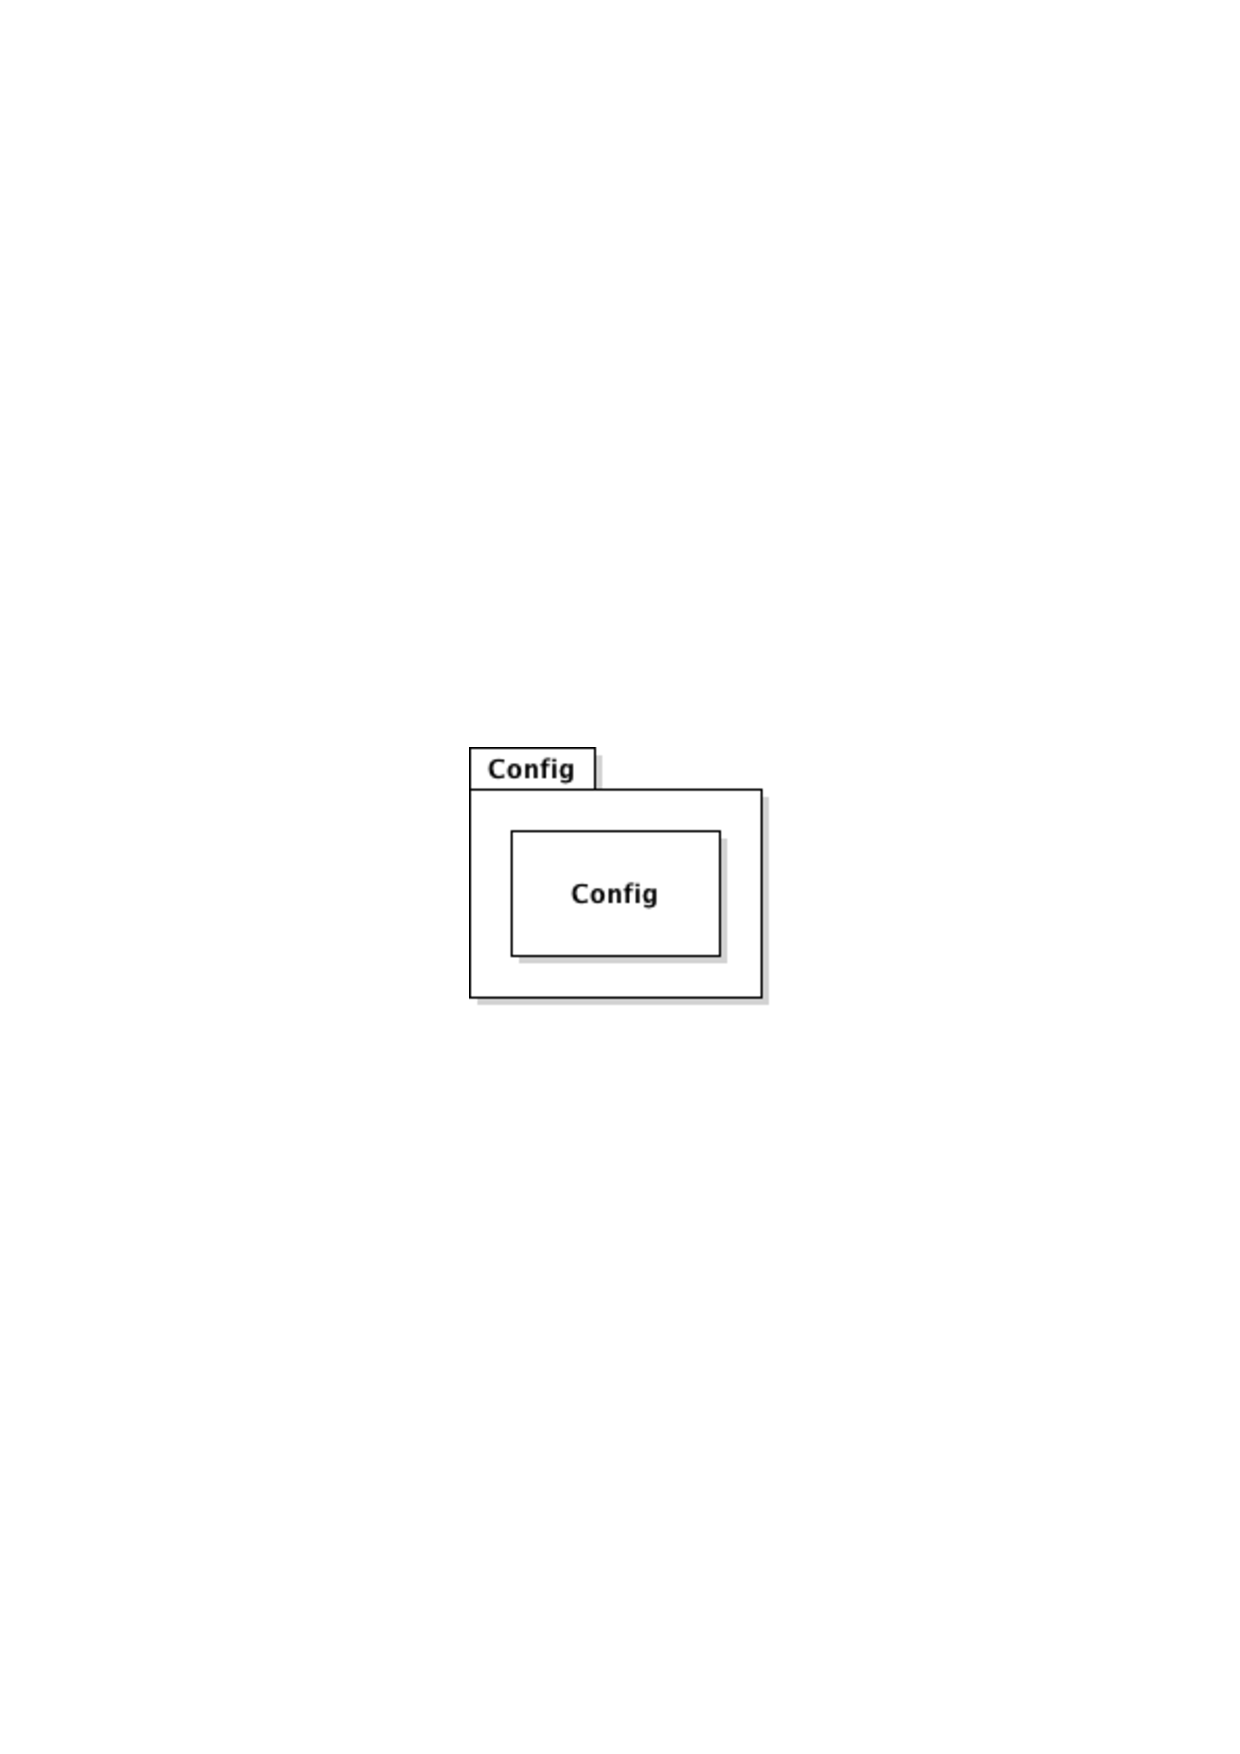
\includegraphics[width=\textwidth,  trim=2cm 12cm 2cm 12cm]{UML_figure/DC/core/config/DC_Config.pdf}
				\caption{Core diagram class : Config}
			\end{center}
		\end{figure}
		\subsubsection{Config}
			This unit implements a set of general rules affecting the server behavior.
	\subsection{VFS (Versioned File System)}
		\begin{figure}[ht]
			\begin{center}
				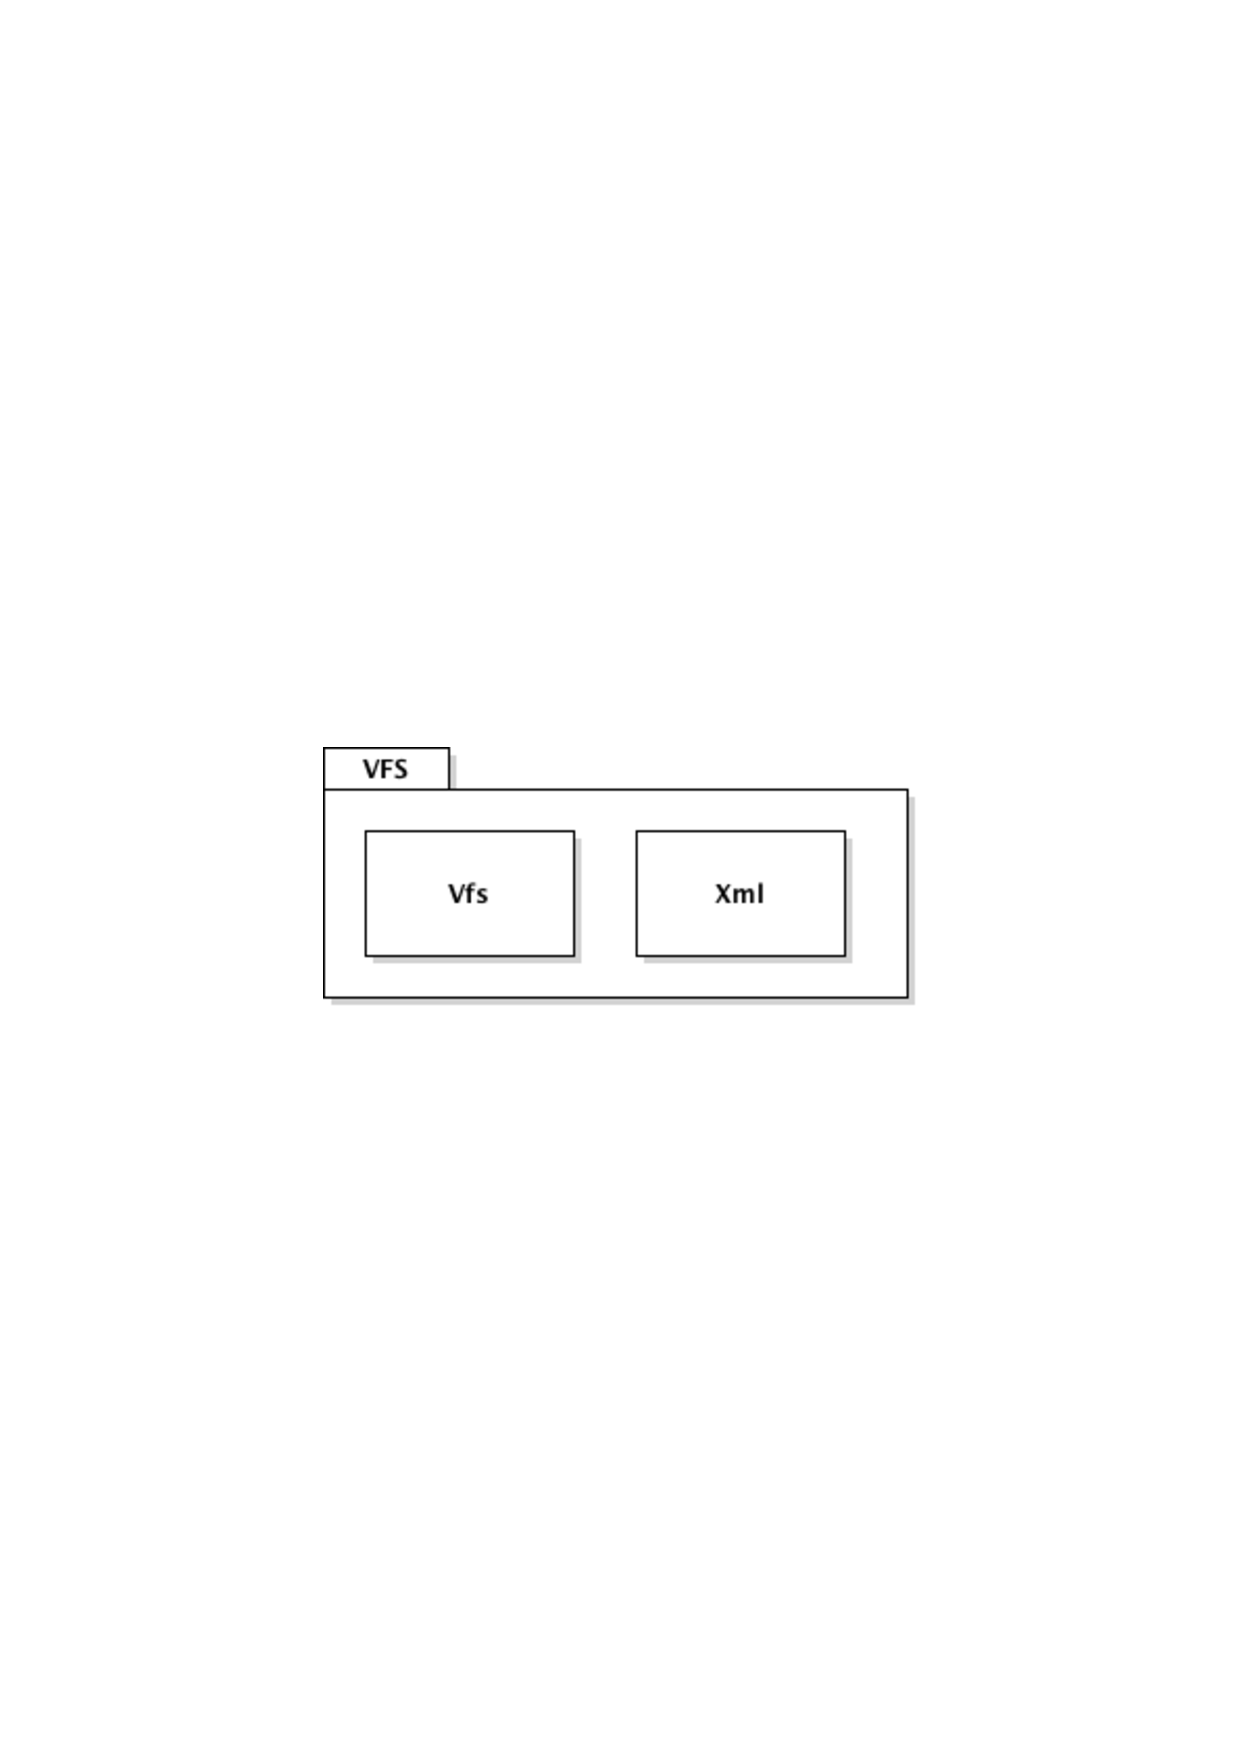
\includegraphics[width=\textwidth,  trim=2cm 12cm 2cm 12cm]{UML_figure/DC/core/vfs/DC_VFS.pdf}
				\caption{Core diagram class : VFS}
			\end{center}
		\end{figure}
		\subsubsection{VFS}
			This module implements a versioned hierarchical file system.
		\subsubsection{XML}
			This unit implements a XML parser.
\newpage
	\subsection{Common}
		\begin{figure}[ht]
			\begin{center}
				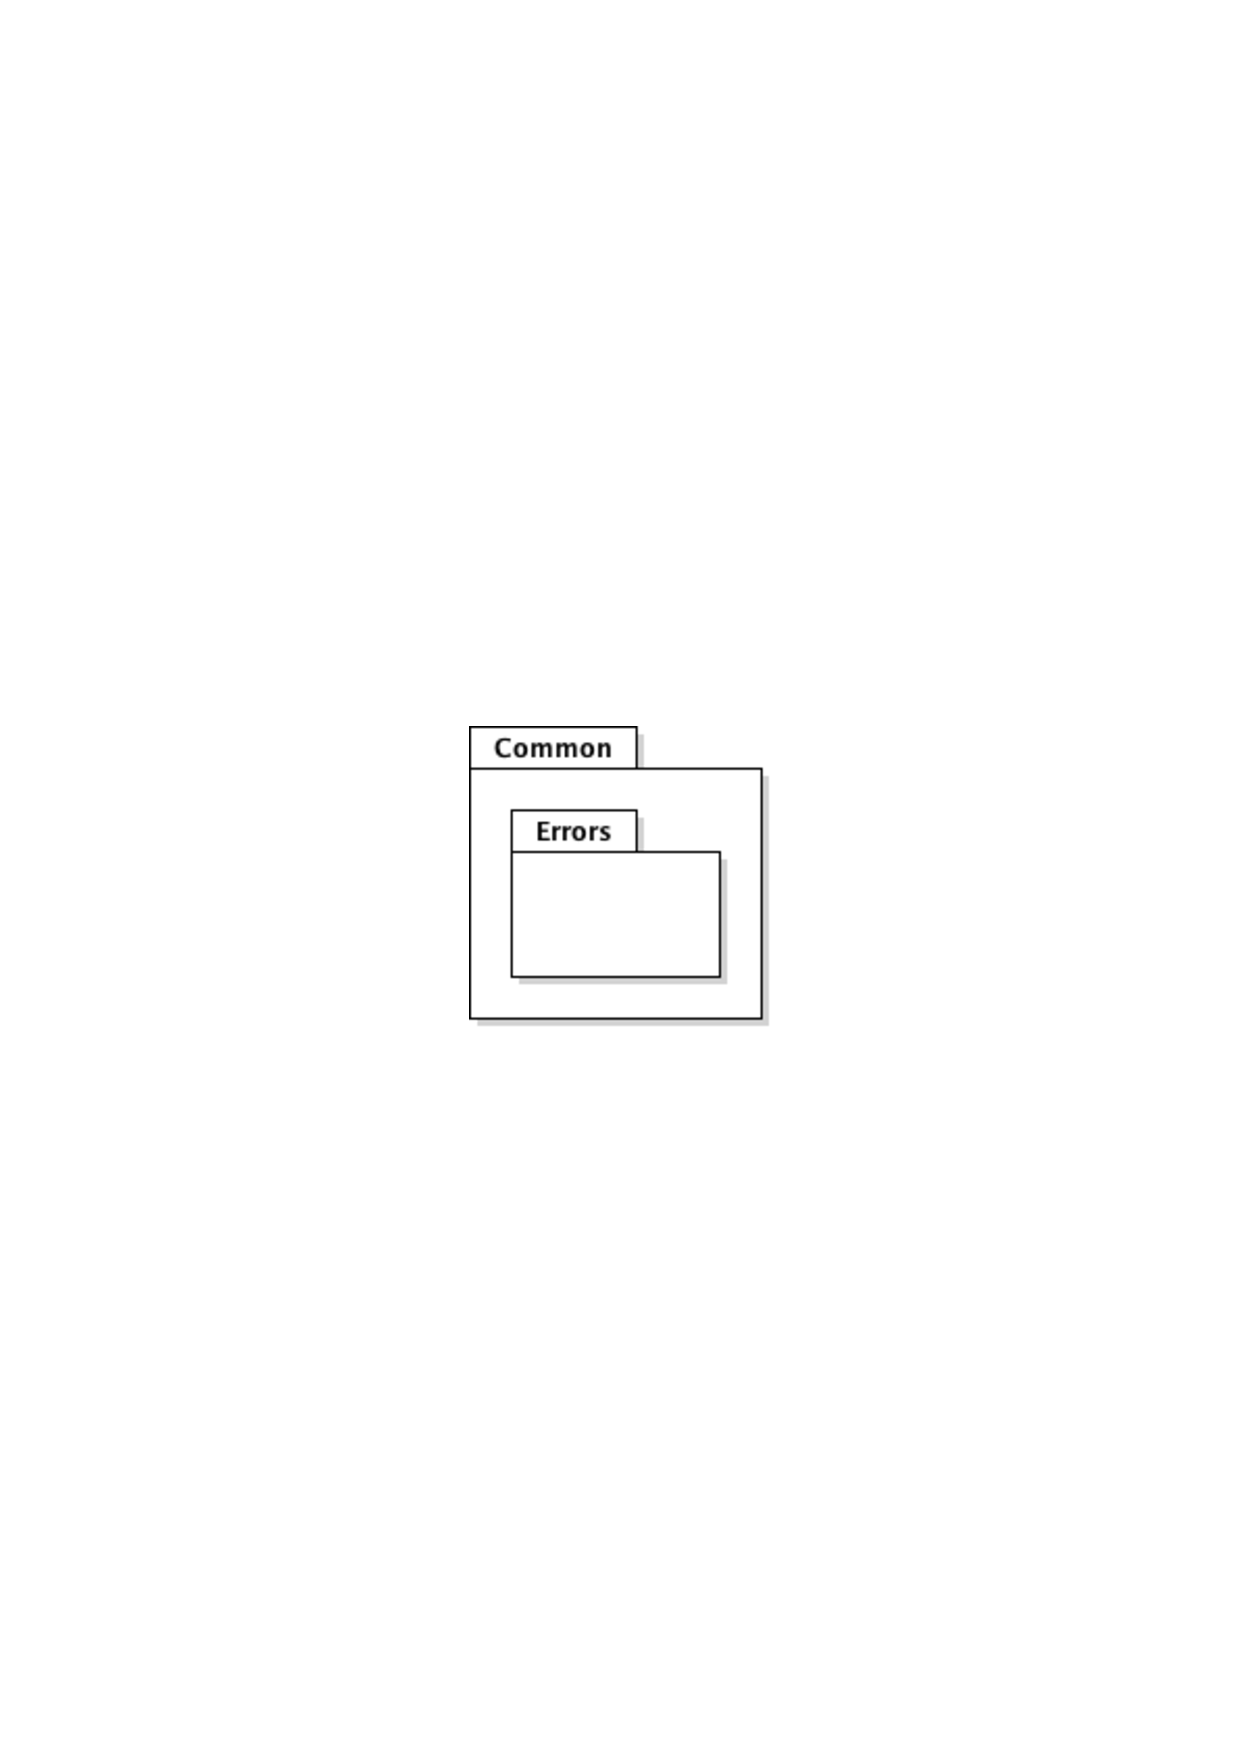
\includegraphics[width=\textwidth,  trim=2cm 12cm 2cm 12cm]{UML_figure/DC/core/common/DC_Common.pdf}
				\caption{Core diagram class : Common}
			\end{center}
		\end{figure}
	\subsection{Common :  Errors}
		\begin{figure}[ht]
			\begin{center}
				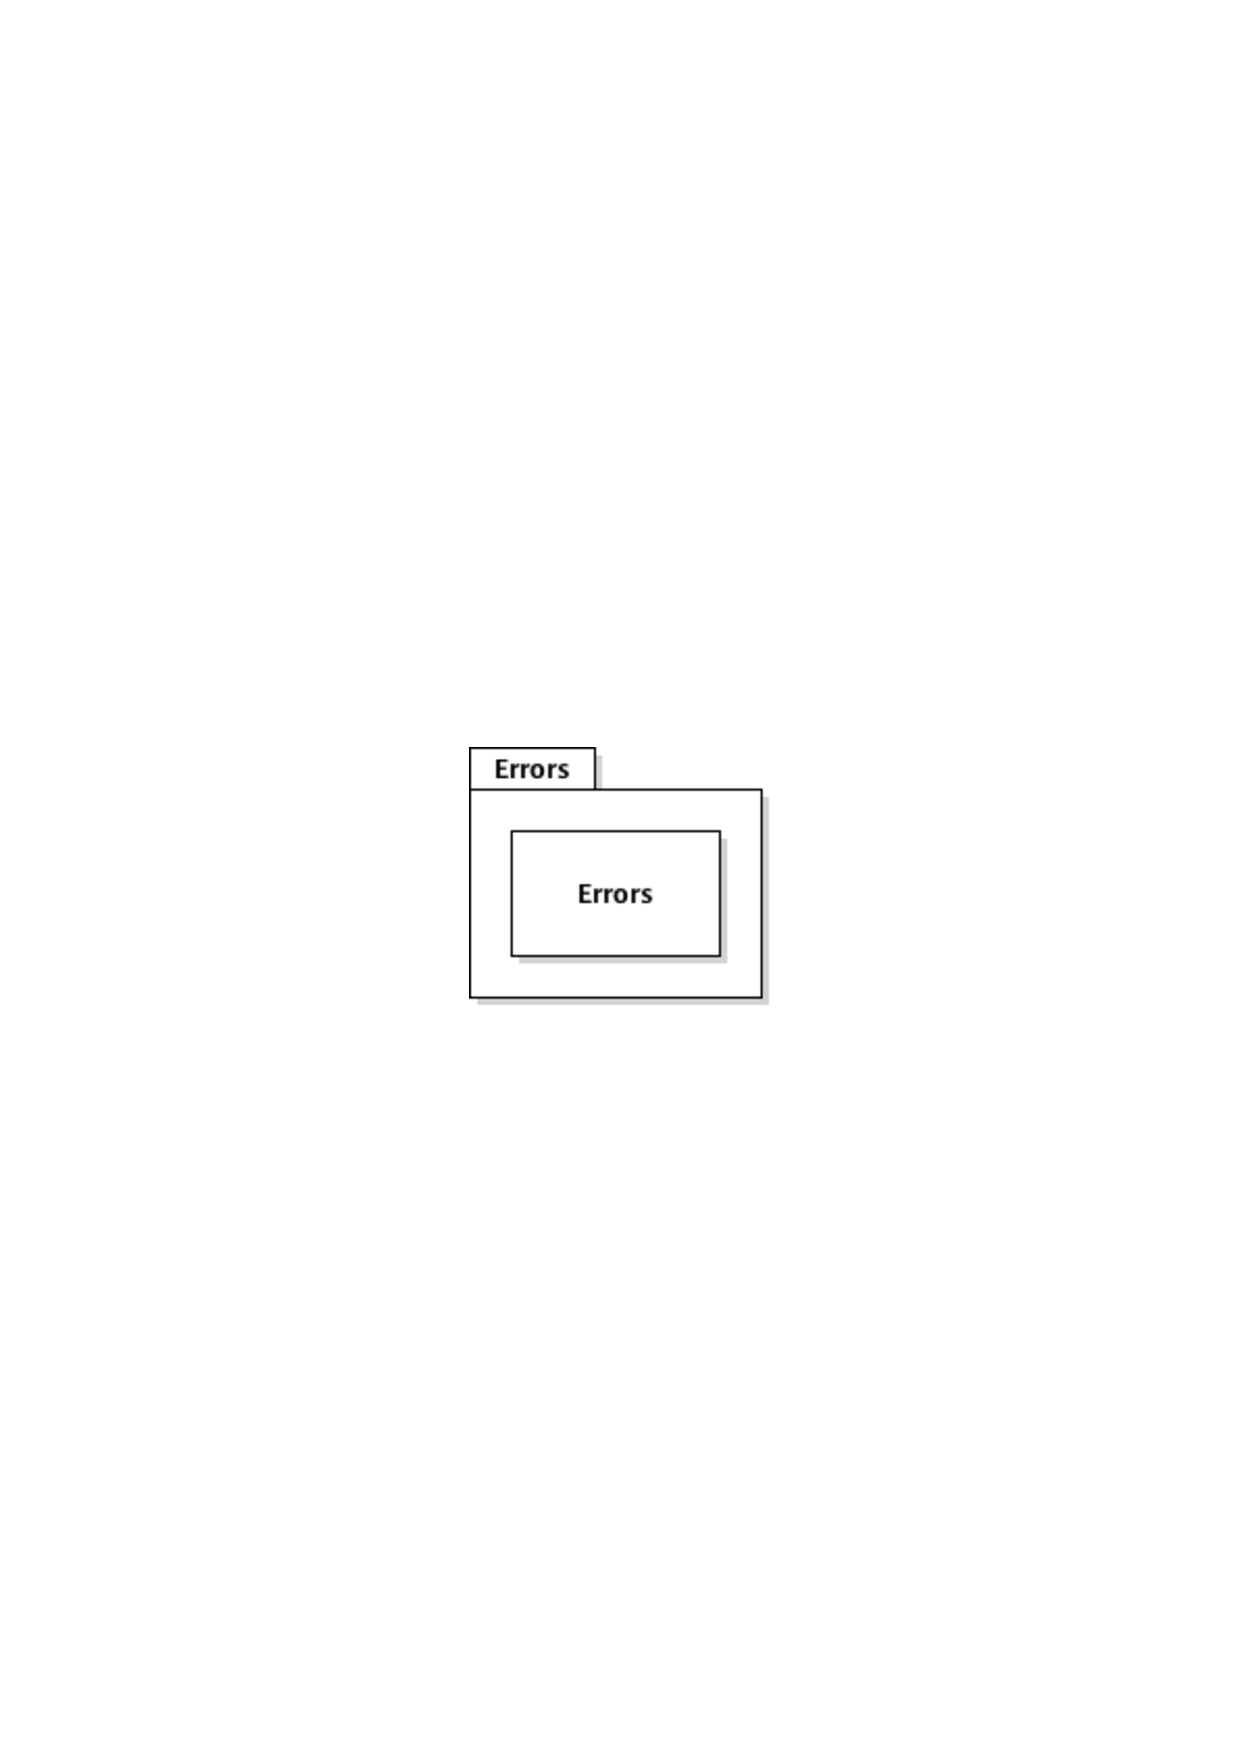
\includegraphics[width=\textwidth,  trim=2cm 12cm 2cm 12cm]{UML_figure/DC/core/common/DC_Errors.pdf}
				\caption{Core diagram class : Common - Errors}
			\end{center}
		\end{figure}
		\subsubsection{Errors}
			This module implements type of exception.
%end core diagram
\newpage
\section{Common}
	\begin{figure}[ht]
			\begin{center}
				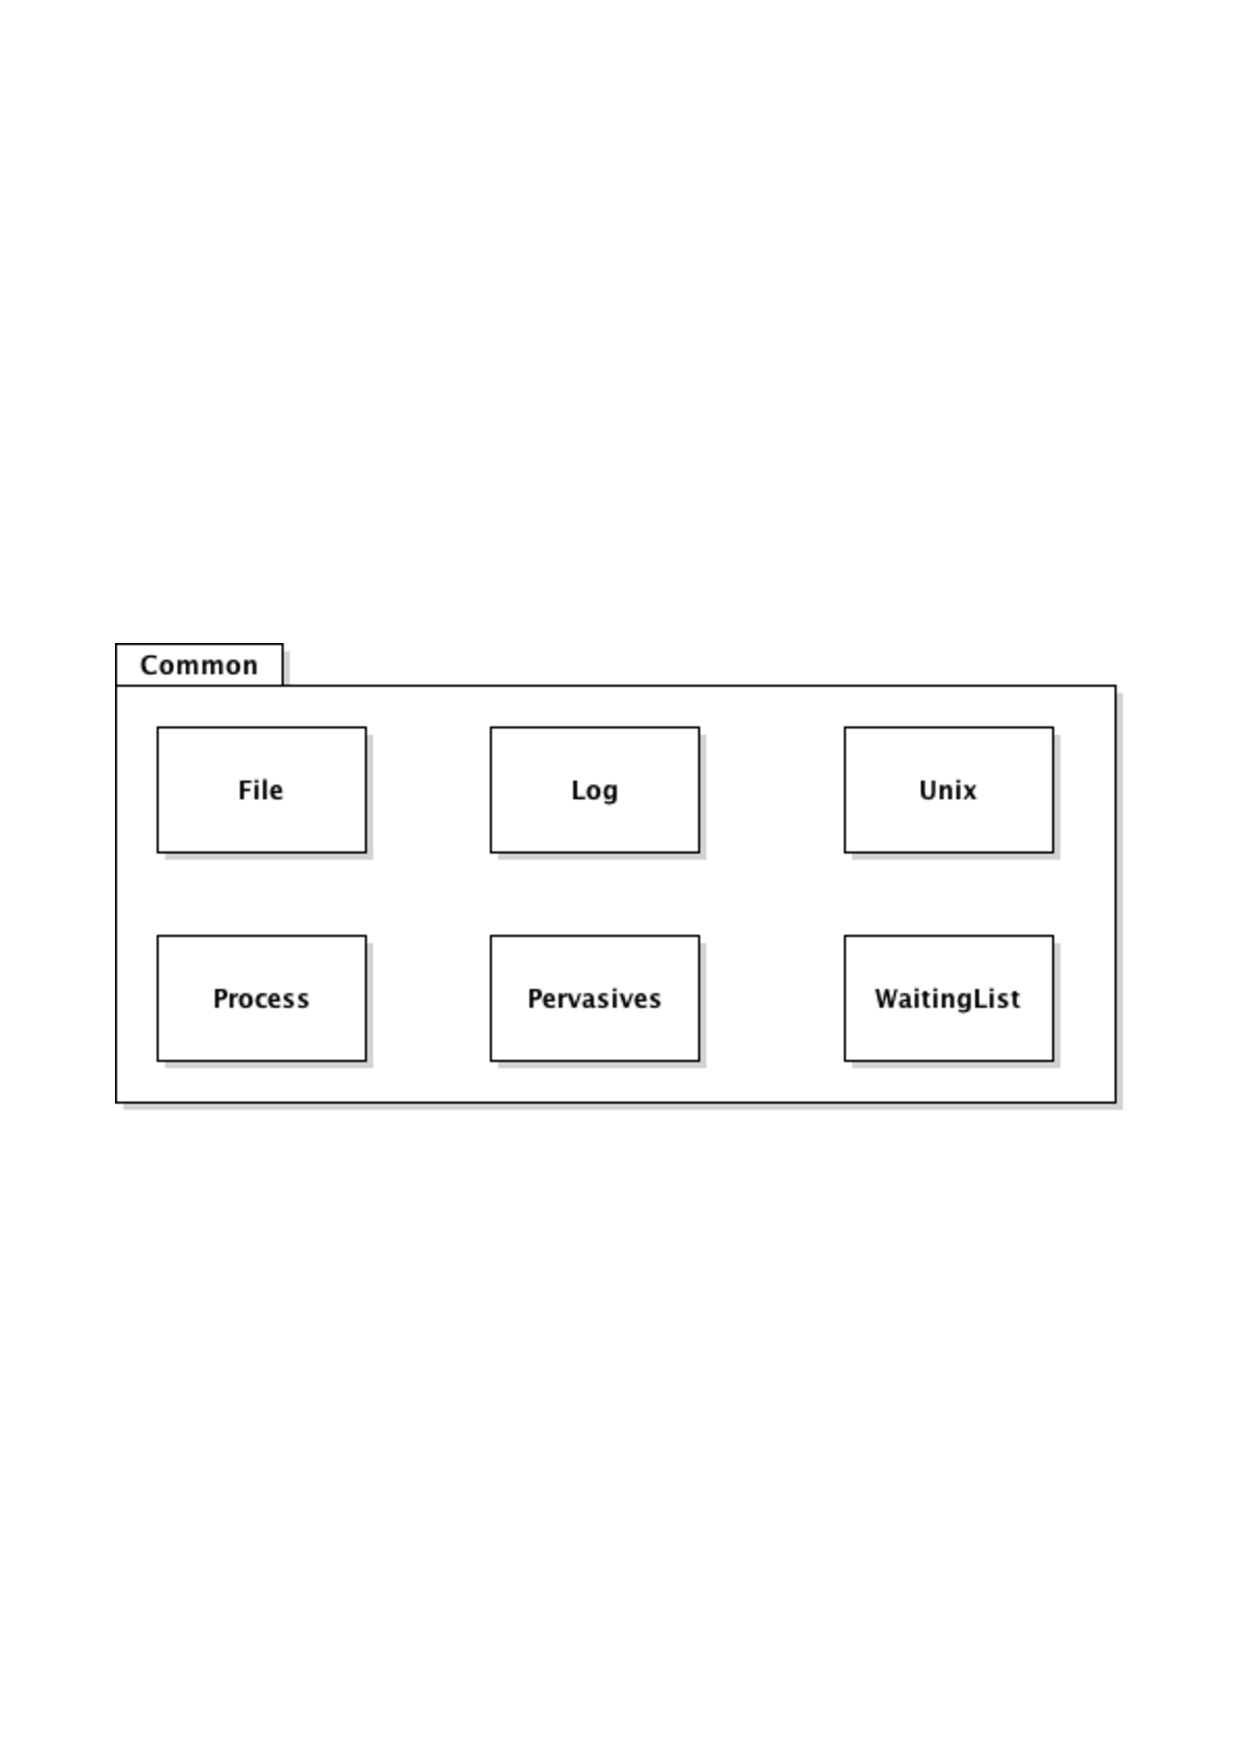
\includegraphics[width=\textwidth,  trim=2cm 10cm 2cm 11cm]{UML_figure/DC/common/DC_Common.pdf}
				\caption{Common diagram class : Overview}
			\end{center}
		\end{figure}







